\chapter{Safety and assurance}

\section{Definition}

Safety is often defined as \cite{organization2018iso}:
\begin{quotation}
Absence of unreasonable risk.
\end{quotation}  
An unreasonable risk is a \cite{organization2018iso}:
\begin{quotation}
Risk judged to be unacceptable in a certain context according to valid societal moral concepts.
\end{quotation}
Various safety standards have been developed for different industries and activities. Some examples are ISO 26262 for functional safety of road vehicles, DO-178C for aerospace industry, ISO 8124 for safety of toys, ISO 7164 for healthcare organization management.

\section{Safety Assurance Case}

Assurance cases have been successfully used in various industries to describe why a system can be trustfully used for a specific application \cite{Ashmore2021}.
A recent definition of safety assurance case is described in \cite{Bloomfield2010} as


\begin{displayquote}[][]
"A structured argument, supported by a body of evidence, that provides a compelling, comprehensible and valid case that a system is safe for a given application in a given environment"
\end{displayquote}
A structured argument is a \cite{Omg2010}
\begin{displayquote}[][]
"connected series of statements or reasons intended to establish a position...; a process of reasoning."
\end{displayquote}
Reasons used in a structured argument can be considered as premises in logical terms and a conclusion can be drawn based on them \cite{Omg2010}.  
% A safety assurance case \textcolor{red}{(Assurance case in short)} justifies safety of a system by bringing a valid argument that a set of claims are justified, given that a set of assumptions are fulfilled \cite{Burton}.
The purpose of using an assurance case is to communicate a clear, comprehensive, defensible argument that a system is safe to be used in a particular context \cite{gsn2004Kelly}. Assurance cases are comprised of five basic components: claims, arguments, evidence, justifications and assumptions. The most common use of assurance cases is to give assurance about system's functionality and properties to the parties which were not involved in the process of developing the system \cite{iso15026-1-2019}.

Assurance cases reason in a subjective manner, as compared to the logical proofs which consider an absolute truth. In other words, assurance cases are useful because the full range of a system's properties are not always representable in a logical formalization. Also, assurance cases may sometimes be disproved because the underlying logical theory used in them is not relevant \cite{iso15026-1-2019}.

Since assurance cases are considered artefacts, they inherit quality related properties of them such as: the structure of its content, semantic features such as completeness, creation and maintenance. The conclusions of the assurance case should also be stated clearly with clear level of uncertainty \cite{iso15026-1-2019}. \textcolor{red}{more from 15020 about assurance cases?}

\section{Goal Structuring Notation}
When the safety assurance case is more complex in nature, textual representation suffers to express the case in a clear and understandable way. Figure \ref{fig:text-case} shows an example of such problem where the English structure of the argument is hard to understand. Having multiple cross references is specially difficult to capture in text \cite{gsn2004Kelly}.
\begin{figure}
    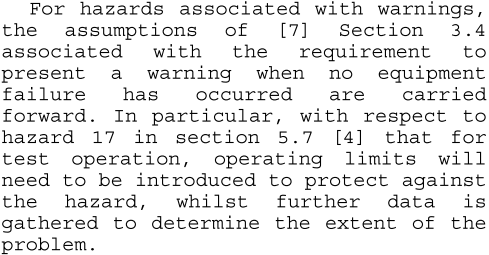
\includegraphics[width=0.5\linewidth ]{figures/textual_case.png}
    \centering
    \caption{Problems associated with textual representation \cite{gsn2004Kelly}.}
    \label{fig:text-case}
\end{figure}

The Goal Structuring Notation(GSN) is a graphical notation for safety argumentation. A GSN explicitly represents elements of a safety argument and the relationships among these components. For example, how requirements are supported by claims or how claims are supported by evidence or how the case has a defined context \cite{gsn2004Kelly}. Figure \ref{fig:gsn} depicts basic building blocks of a GSN with example instances of each element. 

\begin{figure}
    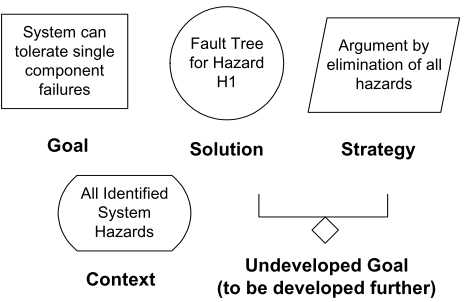
\includegraphics[width=0.5\linewidth ]{figures/gsn.png}
    \centering
    \caption{Basic elements of a GSN \cite{gsn2004Kelly}.}
    \label{fig:gsn}
\end{figure}

\section{An example of a GSN}

The goal structure is used to show how goals (claims about the system) can be split into sub-goals successively until the sub-goal can be directly supported by available evidence. Figure \ref{fig:gsn-example} represents an example of a GSN.

\begin{figure}
    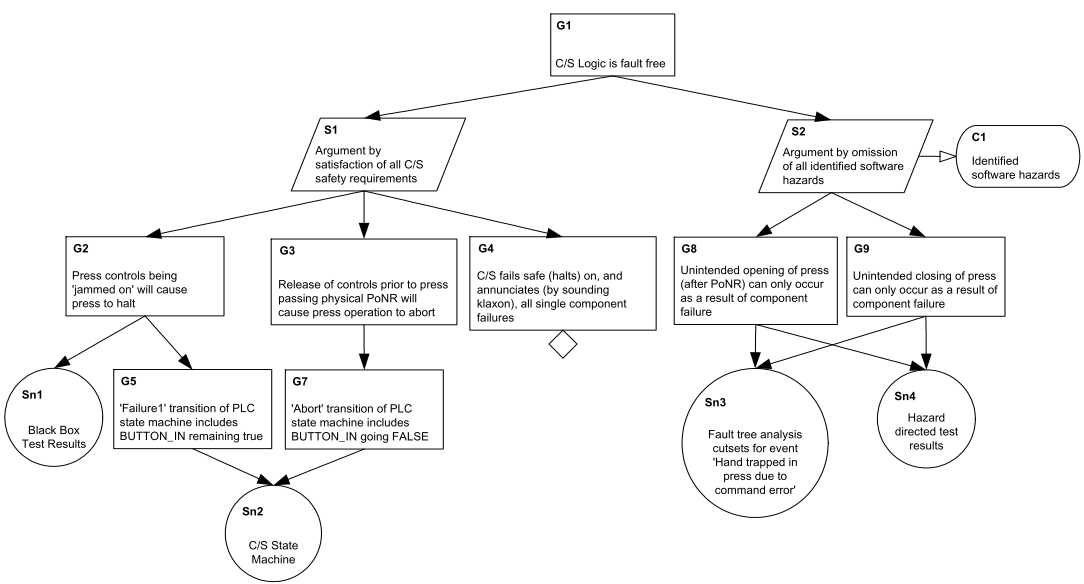
\includegraphics[width=0.9\linewidth ]{figures/gsn-example.png}
    \centering
    \caption{An example of a goal structure \cite{gsn2004Kelly}.}
    \label{fig:gsn-example}
\end{figure}

In this example, "Control System (C/S) logic is fault free." is one single top level goal. The main goal is then divided to two sub-goals through strategies $S1$ and $S2$. These two strategies are then supported by five sub-goals $G2-G4$ and $G8-G9$. In a goal structure, there will be a stage where the sub-goals can be directly supported by solutions. In this example, sub-goals $G8-G9$ are supported by $Sn3-Sn4$ and there is no need to break down the goals further in this branch \cite{gsn2004Kelly}.\\
\textcolor{red}{write about CAE(Claims Arguments Evidence)}
